% 第 18 题立体几何图（五顶点多面体）：按固定源 PDF 矢量路径换算（1 pt → 0.03515 cm）。
% 原点取顶点 A（源页 (263.29, 579.67) pt，即源变换矩阵 tx,ty），y 向上。
% 顶点：A(0,0)、B(126.23,0)、C(53.00,−59.74)、E(28.91,73.23)、F(106.96,91.54)；
% 辅助点 D 为 AC 中点 (26.50,−29.87)、G 为 EC 中点 (40.955,6.745)、H 为 FB 中点 (116.595,45.77)。
% 实线 7 段：轮廓五边形 A-E-F-B-C 与内部 C-E、C-F；虚线 4 段：隐藏棱 A-F、A-B 与辅助线 B-D、G-H。
% 注：G-H 实绘端点相对精确中点偏移 ≤0.5 pt（源内即如此），照源复刻；无箭头。
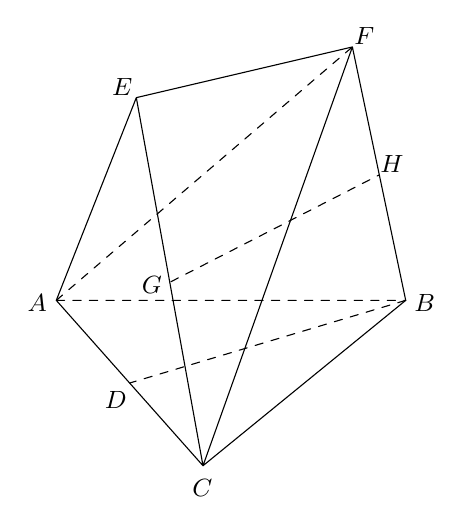
\begin{tikzpicture}[line cap=round,line join=round,font=\small,x=0.03515cm,y=0.03515cm]
% ===== 虚线先画（隐藏棱与辅助线）=====
\draw[dash pattern=on 2.99pt off 2.99pt]
  (0,0)--(106.96,91.54)          % A-F（隐藏棱）
  (0,0)--(126.23,0)              % A-B（隐藏棱）
  (126.23,0)--(26.50,-29.87)     % B-D（辅助线）
  (41.43,6.74)--(116.59,45.29);  % G-H（辅助线，照源实测端点）
% ===== 实线 =====
\draw
  (0,0)--(28.91,73.23)           % E-A
  (28.91,73.23)--(106.96,91.54)  % F-E
  (106.96,91.54)--(126.23,0)     % B-F
  (126.23,0)--(53.00,-59.74)     % C-B
  (53.00,-59.74)--(0,0)          % A-C
  (53.00,-59.74)--(28.91,73.23)  % C-E
  (53.00,-59.74)--(106.96,91.54);% C-F
% ===== 标注（照源字形框中心，显式坐标）=====
\node[anchor=center,inner sep=0] at (-6.87,-1.08) {\(A\)};
\node[anchor=center,inner sep=0] at (133.09,-1.08) {\(B\)};
\node[anchor=center,inner sep=0] at (52.74,-67.82) {\(C\)};
\node[anchor=center,inner sep=0] at (23.79,77.11) {\(E\)};
\node[anchor=center,inner sep=0] at (111.30,95.43) {\(F\)};
\node[anchor=center,inner sep=0] at (21.53,-35.89) {\(D\)};
\node[anchor=center,inner sep=0] at (34.58,5.67) {\(G\)};
\node[anchor=center,inner sep=0] at (121.25,49.16) {\(H\)};
\end{tikzpicture}
